\section{Encoding the action-space}
The output layer of the neural network represents the action space, directly corresponding to one or more Q-values. In the most simple cases where the action space is constant (i.e., for every state, the same actions can be taken regardless of any internal variable values) it is common to output a Q-value for every action. This way all relevant Q-values to decide the next action are calculated at once, and the $argmax$ of the maximum Q-value is the optimal action. The input of the neuron network is a state, the output is a series of Q-values for every possible action in that state.
Contrary to regular Q-learning where we are able to expand an ever-increasing Q-table with state-action pairs, the size of the neural network (including the size of the output layer) has to be predefined before the training process. Deep Q-learning is often applied to environments with a constant action space, where its dimensionality is independent of the input state. This is common for games or well-known optimization problems like ``CartPole'', where all transitions (e.g., move left, move right) are always enabled. In the domain of model checking this is untrue in most cases, the enabled transitions vary for the state of the automaton and the values of the state variables which determine the guard values. An alternate method of encoding the action space is therefore to disregard the convention of multiple Q-values as output, and to encode the complete state-action pair as the input layer. The output of the neural network then becomes a single Q-value. In the following section the difficulties in encoding the action-space and the advantages and disadvantages of various methods of encoding the action space are discussed.

\subsubsection{Parallel composition}
A model can contain multiple parallel automatons, each automaton is in a certain state and has a certain value for the variables allocated in its namespace. The scheduler can then choose an action for any of the automatons, and depending on the values of its variables and the predefined synchronization vectors, multiple automatons can synchronize. One possible solution for the problem of action-space encoding is the record the largest number of possible commands an automaton can make for any given state it can be in and set the number of output neurons equal to that number. For any given state at any given time we then order the possible commands in a constant manner. However, for a model containing more than one automaton, it is ambiguous to which action the output neurons correspond to; i.e., which scheduler do we choose? Creating a different neural network for the different automatons is not a solution either because we are interested in the interplay between the behaviors and variables in each automaton.

\subsubsection{Process synchronization}
In an MDP with multiple independent automatons there exists the possibility for multiple transitions two synchronize. When this occurs all automatons are advanced to the future state in accordance with their appropriate $(s, t, s')$ tuple. Whether and when a transition of a given automaton can synchronize with the transitions of another automaton depends on the synchronization vectors. Given a synchronization vector $(\alpha, -, \beta, \tau)$, automaton $0$ is able to synchronize transition label $\alpha$ with automaton $2$ with transition label $\beta$ and automaton $3$ with transition label $\tau$. However, given one of said automatons, there can be no or multiple transitions enabled with the transition label required for synchronization. Encoding all possible permutations in the action space as a single action each poses the problem of a possible action-space explosion. When encoding the different possible options all falling under the same synchronization vector as the same action will not yield accurate results as action with the same label yet different futures (can) yield different rewards.

\subsection{Solutions}
When considering a model encoded in the JANI\cite{jani} or Modest\cite{modest} format, the label given to an action has no particular meaning other than human-readability and synchronization. The transition label itself does not provide ample distinction as the model checker allows for an overlap in the transition labels. For example, for a given state there can be multiple outgoing transitions with label $a$, and this label can occur in multiple different automatons. There is no connection between the transitions all identifying as $a$, and training the model in a way that does not discern between these transitions can yield incorrect results. For regular Q-learning this does not pose a problem as we can simply record the command for this specific state in the Q-table, there is no definition collision between this action for this state with similar actions in other states. Furthermore, for a given transition there can be multiple enabled guards in case the guard conditions are overlapping. In this case there are multiple transitions applicable for a given transition label in a state for a given set of variables that are evaluated against a set of guard expressions. Because of this discrepancy between regular Q-learning and Deep Q-learning the output layer should be encoded to account for the varying action space. To achieve this, one can consider multiple potential solutions.

\subsubsection{One-to-one mapping of neurons and commands}
If we consider every command (specifically discerning between overlapping guard expressions like $k \ge 0$ and $k = 0$ which collide at $k = 0$) we end up with a unique output neuron for every possible action the model can take. This means we end up with an action space that grows exponentially with the number of states, as every action in every state adds $n$ actions to the output layer. When considering fully connected layers between the output neurons and the rest of the network this quickly becomes unfeasible when optimizing for large models, and a regular Q-table would be more efficient and more accurate. Additionally we need to consider the problem of choosing a correct action; the output layer contains the predicted Q-values for every action. This includes Q-values for actions which are non-applicable in the state of interest. This is not the case for models with a constant action space and in regular Q-learning, in these cases every Q-value and matching action in the output layer or Q-table can be considered at all times. If we only select a very small subset of the output layers' data, the model will not learn what to do with most neurons in most cases as it's only being tested against some of its outputs at one particular time. There may even be output neurons which are (nearly) never used or validated against because of the chosen scheduler.

\subsubsection{Flattened model representation}
A possible solution to the issues arising from synchronization is to consider the flattened MDP model instead. Here all the behavior of the individual automatons is expressed as a single main automaton. This has the advantage of not having to account for the different possible transitions required for a transition to synchronize. However, this approach has several caveats. For one, the model that results from the flattening is more complex than the original model. Ideally, there is a method of encoding the state-action pair and its subsequent Q-value in such a way that a non-flattened model would suffice. The behavior of a simple clock, for example, which dictates whether a transition can be taken in another automaton is now embedded in a more complex main automaton.

Flattening the model results in a single automaton that is strongly bisimilar to the behavior of the separate original automatons. The main advantage of this approach is the negation of the synchronization between the individual automatons, and the simpler encoding of the action space it enables. It also reduces the number of overlapping actions caused by synchronization. For example, if action $a$ in automaton $0$ and action $b$ in automaton $1$ are included in the same synchronization vector, choosing either action will have the same effect on the network; automaton $0$ will take transition $a$ and automaton $1$ will take transition $b$. In the flattened model it is no longer ambiguous which automaton should be addressed, and there is no overlap in actions between different network components.

If we now consider the maximum number of actions in any location, which can be easily extracted from the flattened model, to be the size of the action space we have a significantly smaller array of options.

\begin{figure}[h]
    \centering
    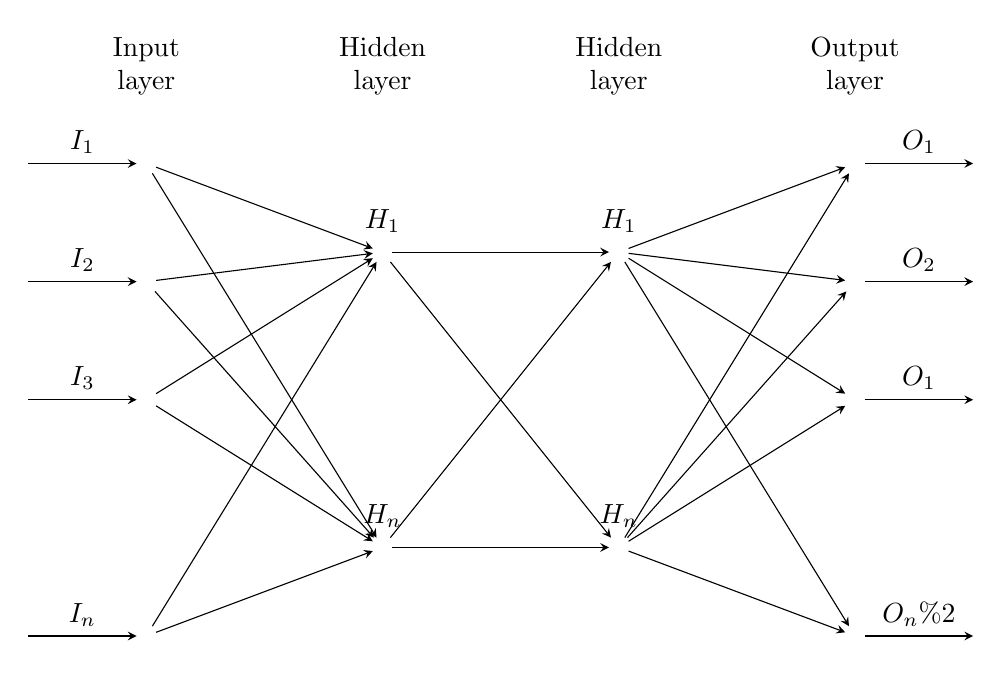
\begin{tikzpicture}[x=1.5cm, y=1.5cm, >=stealth]
    
    \foreach \m/\l [count=\y] in {1,2,3,missing,4}
      \node [every neuron/.try, neuron \m/.try] (input-\m) at (0,2.5-\y) {};
    
    \foreach \m [count=\y] in {1,missing,2}
      \node [every neuron/.try, neuron \m/.try ] (hidden0-\m) at (2,2-\y*1.25) {};
    
    \foreach \m [count=\y] in {1,missing,2}
      \node [every neuron/.try, neuron \m/.try ] (hidden1-\m) at (4,2-\y*1.25) {};
    
    \foreach \m [count=\y] in {1,2,3,missing,4}
      \node [every neuron/.try, neuron \m/.try ] (output-\m) at (6,2.5-\y) {};
    
    \foreach \l [count=\i] in {1,2,3,n}
      \draw [<-] (input-\i) -- ++(-1,0)
        node [above, midway] {$I_\l$};
    
    \foreach \l [count=\i] in {1,n}
      \node [above] at (hidden0-\i.north) {$H_\l$};
    
    \foreach \l [count=\i] in {1,n}
      \node [above] at (hidden1-\i.north) {$H_\l$};
    
    \foreach \l [count=\i] in {1,2,1,n \% 2}
      \draw [->] (output-\i) -- ++(1,0)
        node [above, midway] {$O_\l$};
    
    \foreach \i in {1,...,4}
      \foreach \j in {1,...,2}
        \draw [->] (input-\i) -- (hidden0-\j);
    
    \foreach \i in {1,...,2}
      \foreach \j in {1,...,2}
        \draw [->] (hidden0-\i) -- (hidden1-\j);
    
    \foreach \i in {1,...,2}
      \foreach \j in {1,...,4}
        \draw [->] (hidden1-\i) -- (output-\j);
    
    \foreach \l [count=\x from 0] in {Input, Hidden, Hidden, Output}
      \node [align=center, above] at (\x*2,2) {\l \\ layer};
    
    \end{tikzpicture}
    \caption{Graphical representation of a neural network with $n$ output neurons, where the associated action $a$ for a location with $2$ actions corresponds to output neurons where $n \% 2 = a$.}
    \label{fig:nn_mod}
\end{figure}

We can then encode the actions in such a way that there is not a possibility for an ``invalid transition'', i.e. an action which is not enabled in the current state, to be taken at any moment. This is achieved by computing the modulo of the output neuron index with respect to the number of enabled actions in the current state (e.g., figure \ref{fig:nn_mod}). The resulting action index will always have a corresponding enabled action. However, there is a scalar of issues that arises from this approach. The first and foremost issue is caused by guards and their effect on the enabled transitions. If we consider an MDP where the number of enabled actions depends on the value of a state variable (e.g., figure \ref{fig:mdp_enabled_action_count}) we encounter a problem if we encode and decode the action based on the number of enabled actions. In this figure action $a$ is either not listed as an enabled action when $k = 0$, or listed as an enabled action after the network has traversed to $s_1$ via action $b$ and back to $s_0$ via action $\tau$ at least once, resulting in the guard $k > 0$ being satisfied.

\begin{figure}
    \centering
    \begin{tikzpicture}[auto,node distance=8mm,>=latex,font=\small]
        \tikzstyle{round}=[thick,draw=black,circle]
        
        \node[round] (s0) {$s_0$};
        \node[round,above right=0mm and 40mm of s0] (s1) {$s_1$};
        \node[round,below right=0mm and 40mm of s0] (s2) {$s_2$};
        
        \draw[->] (s0) -- node[above] {$b$} (s1);
        \draw[->] (s1) [out=160,in=20] to node[above] {$\tau$, $k \leftarrow k + 1$} (s0);
        \draw[->] (s0) -- node[above] {$c$} (s2);
        \draw[->] (s0) [out=40,in=100,loop] to node[above] {$a$ [$k > 0$]} (s0);
    \end{tikzpicture}
    \caption{MDP for which the action space size is $2$ for $k = 0$ and $3$ for $k > 0$, this poses a challenge to encoding the action space in a neural network as action $b$ could potentially be mapped to either output neuron $1$ or output neuron $2$, depending on the value of $k$.}
    \label{fig:mdp_enabled_action_count}
\end{figure}

\subsubsection{Single Q-value action-space}

If we instead flip the convention of outputting a Q-table after entering the current state as the input layer, and instead output a single Q-value given an observation and action we get a neural network more akin to the mathematical representation of Q-learning. In the mathematical model one considers state-action pairs to be the \emph{key} in the Q-table, and the Q-value to be the \emph{value}. This means the action space needs to be \emph{encoded} in the input layer and therefore does not need to be \emph{decoded} in the output layer.

Having only one output neuron solves several issues considered and touched upon in the sections before. Due to the fact that we are not selecting actions from a table anymore, the possibility of selecting a Q-value belonging to an action not in the action space of the current state is not applicable anymore. Any information we feed into the network (given it is valid information), returns a singular Q-value.

Because the action needs to be encoded in the input layer, new problems arise. For one, the number of input neurons is increased, and as a result the network may be overstimulated in its process to find the correct weights in its optimization efforts. There are several methods of encoding the action space into the input layer. The most straightforward method is to use a similar approach to what was done in decoding the output layer; to consider the enabled actions in a given state and encode the index of this action (either ordinal or one-hot) as the input neuron. This solution worked well for the output layer encoding because we are not in control of what the network outputs, however we \emph{are} in control of what we feed into the network.

This opens the possibility of feeding the raw transition data directly into the network. These are the transition tuples the network in the Modest Python export considers, in which a transition number always corresponds to a single transition for every separate automaton. The behavior of all automatons is encoded in any transition tuple, and therefore process synchronization can be expressed as well. Given this tuple of transitions is gained by querying the network, the tuple is always valid and its transitions are therefore enabled.

\begin{figure}[h]
    \centering
    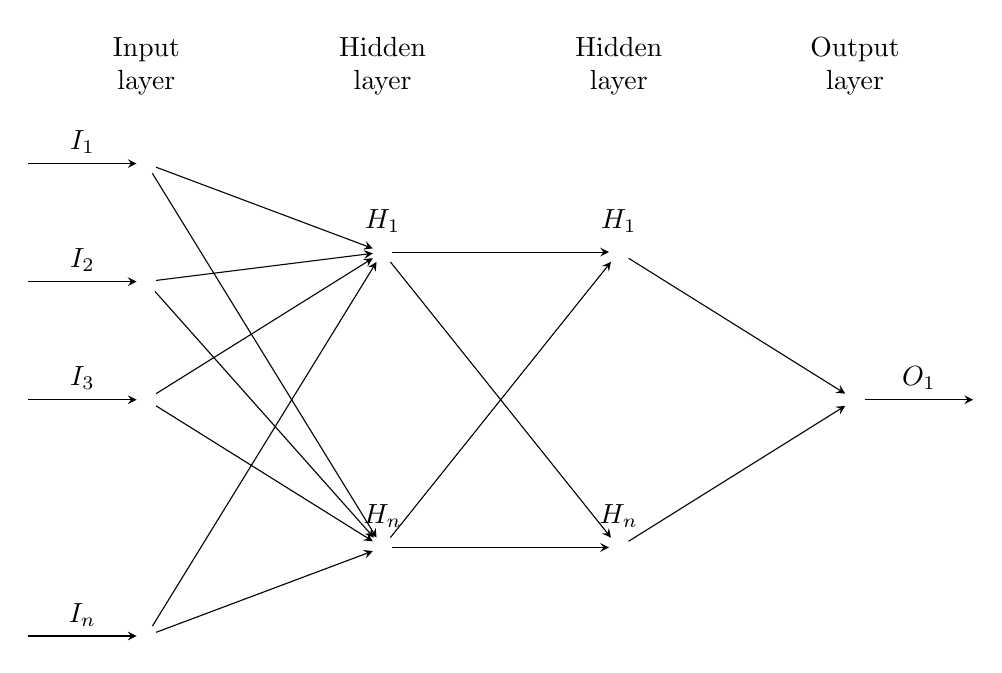
\begin{tikzpicture}[x=1.5cm, y=1.5cm, >=stealth]
    
    \foreach \m/\l [count=\y] in {1,2,3,missing,4}
      \node [every neuron/.try, neuron \m/.try] (input-\m) at (0,2.5-\y) {};
    
    \foreach \m [count=\y] in {1,missing,2}
      \node [every neuron/.try, neuron \m/.try ] (hidden0-\m) at (2,2-\y*1.25) {};
    
    \foreach \m [count=\y] in {1,missing,2}
      \node [every neuron/.try, neuron \m/.try ] (hidden1-\m) at (4,2-\y*1.25) {};
    
    \foreach \m [count=\y] in {1}
      \node [every neuron/.try, neuron \m/.try ] (output-\m) at (6,0.5-\y) {};
    
    \foreach \l [count=\i] in {1,2,3,n}
      \draw [<-] (input-\i) -- ++(-1,0)
        node [above, midway] {$I_\l$};
    
    \foreach \l [count=\i] in {1,n}
      \node [above] at (hidden0-\i.north) {$H_\l$};
    
    \foreach \l [count=\i] in {1,n}
      \node [above] at (hidden1-\i.north) {$H_\l$};
    
    \foreach \l [count=\i] in {1}
      \draw [->] (output-\i) -- ++(1,0)
        node [above, midway] {$O_\l$};
    
    \foreach \i in {1,...,4}
      \foreach \j in {1,...,2}
        \draw [->] (input-\i) -- (hidden0-\j);
    
    \foreach \i in {1,...,2}
      \foreach \j in {1,...,2}
        \draw [->] (hidden0-\i) -- (hidden1-\j);
    
    \foreach \i in {1,...,2}
      \foreach \j in {1,...,1}
        \draw [->] (hidden1-\i) -- (output-\j);
    
    \foreach \l [count=\x from 0] in {Input, Hidden, Hidden, Output}
      \node [align=center, above] at (\x*2,2) {\l \\ layer};
    
    \end{tikzpicture}
    \caption{Graphical representation of a neural network with $1$ output neuron, where the both the state and action is encoded in the input layer.}
    \label{fig:nn_single_q}
\end{figure}